% Apêndice E1 do artigo E4: caderno de especificação de design.
% Entra depois das referências do E4 e usa a mesma lista de referências.
\clearpage
\twocolumn[{\centering
{\Large\bfseries Apêndice E1 --- Caderno de especificação de design}\\[4pt]
{\small Anexo ao artigo E4, fora do limite de oito páginas. As citações remetem às referências do artigo.}\\[6pt]
\hrule\vspace{10pt}}]
\renewcommand{\thetable}{E\arabic{table}}\setcounter{table}{0}
\renewcommand{\thefigure}{E\arabic{figure}}\setcounter{figure}{0}
\newcommand{\Etitle}[1]{\par\medskip\noindent{\normalsize\bfseries #1}\par\smallskip}

\Etitle{Metamensagem e espaço de design com dois receptores}
\textit{Metamensagem do designer.} Este é o meu entendimento, como designer, de quem você é: uma pessoa que amplia a tela para ler, lê com fluência quando a palavra cabe na vista e pode perder a relação entre um prato e o seu preço. Você quer pedir a sua refeição e conferir a de quem vai comer com você, de preferência comparando antes de decidir e corrigindo antes de registrar, porque um engano só aparece quando a comida chega. Este, portanto, é o sistema que projetei para você: cada escolha reúne nome, opções e preço; você pode voltar a eles, conferir o que já incluiu e corrigir o pedido antes de confirmá-lo; e, quando uma opção não estiver clara, há uma explicação no ponto em que a dúvida surgiu. A interface funciona como preposto do designer \cite[p.~84]{desouza}, e a perspectiva comunicativa admite manipulação direta \cite[p.~230]{barbosa}. A Tabela~\ref{tab:jakobson} decide a equivalência de canal entre os dois receptores.
\begin{table*}[!t]
\caption{Espaço de design com dois receptores (elementos de Jakobson na Engenharia Semiótica)}
\label{tab:jakobson}
\centering\scriptsize\setlength{\tabcolsep}{3pt}\renewcommand{\arraystretch}{1.1}
\begin{tabularx}{\textwidth}{@{}>{\raggedright\arraybackslash}p{.075\textwidth}>{\raggedright\arraybackslash}p{.17\textwidth}>{\raggedright\arraybackslash}X>{\raggedright\arraybackslash}X>{\raggedright\arraybackslash}p{.2\textwidth}@{}}
\hline \textbf{Elemento} & \textbf{Pergunta do designer} & \textbf{Para a persona} & \textbf{Para o agente} & \textbf{Diferença declarada e status}\\ \hline
Emissor & Que limitações e intenções do designer devem ser comunicadas? & O designer se manifesta em preços, opções, respostas e na ajuda; o restaurante é fictício e não processa pagamento. & O mesmo preposto produz a observação seguinte, com os mesmos textos e respostas. & Nenhuma diferença de autoria. PD: autoria comum.\\
Receptor & Que aspectos do usuário, como interpretado pelo designer, devem ser comunicados? & Lívia amplia a tela, pode perder a relação entre prato e preço e quer conferir antes de registrar. & O modelo escolhe uma ação a partir do recorte recebido e da memória limitada de trechos vistos. & O agente não tem a experiência de Lívia. HO: representação funcional da persona.\\
Contexto & Que elementos do contexto o sistema processa, e como? & Reconhece a ocasião (almoço, pedido da irmã, jantar) e lê o combinado na instrução. & Recebe a mesma instrução literal da tarefa. & Ruído, pressa e companhia ficam fora da sessão. HO.\\
Código & Qual é a linguagem de interface? & Português, moeda em reais, etiquetas V/SL/SA, posição, tipografia, cor e controles. & Texto dos fragmentos legíveis, tipo e coordenadas dos elementos. & O agente perde parte das pistas de tipografia e cor. HO.\\
Canal & Por quais canais a metacomunicação chega? & Tela do smartphone vista por uma região ampliada que ela desloca. & Interseções legíveis entre signos e recorte $360/z\times800/z$, com memória FIFO de fragmentos. & Aproximação geométrica da vista ampliada. HO.\\
Mensagem & O que se quer contar, e com que efeito? & Escolher, conferir, corrigir e registrar uma refeição; a confirmação comunica o fim. & A mesma mensagem, recebida pelos mesmos signos e pela mesma confirmação. & O sucesso é decidido pelo verificador externo, nunca pela fala do agente. PD.\\ \hline
\end{tabularx}
\end{table*}



\Etitle{Tabela de paridade de signos}
\noindent O esquema descreve cada signo usado nas tarefas pelo conteúdo e pela expressão. Não é o modelo de dados. A coluna \emph{Na observação do agente} aplica a equivalência de canal: \emph{trecho} é o texto geométrica e tipograficamente legível no recorte; abaixo do limiar de legibilidade restam o tipo do elemento e sua posição. Nenhum identificador interno, estado lógico de desabilitação ou elemento fora do recorte entra na observação. A coluna \emph{Evento} liga o signo ao registro do pesquisador. Os signos de aplicação recebem explicação completa nas três camadas da ajuda.
\newcommand{\SGhead}{\hline \textbf{Signo (entidade.atributo)} & \textbf{Origem} & \textbf{Conteúdo (tipo, restrições, default)} & \textbf{Expressão (widget)} & \textbf{Tipo} & \textbf{Na observação do agente} & \textbf{Evento}\\ \hline}
\begin{table*}[!t]
\caption{Esquema conceitual de signos estendido (parte 1: cardápio, item e navegação)}
\label{tab:signos1}
\centering\scriptsize\setlength{\tabcolsep}{3pt}\renewcommand{\arraystretch}{1.08}
\begin{tabularx}{\textwidth}{@{}>{\raggedright\arraybackslash}p{.135\textwidth}>{\raggedright\arraybackslash}p{.085\textwidth}>{\raggedright\arraybackslash}X>{\raggedright\arraybackslash}p{.15\textwidth}>{\raggedright\arraybackslash}p{.085\textwidth}>{\raggedright\arraybackslash}p{.165\textwidth}>{\raggedright\arraybackslash}p{.13\textwidth}@{}}
\SGhead
Restaurante.nome & domínio & texto; denominação do restaurante ou da lanchonete de treino & cabeçalho & estático & trecho legível & \UXev{elemento_visto}\\
Tela.assunto & aplicação & enumerado S0--S5; cena corrente & título da tela & estático & trecho do título & \UXev{tela_alterada}\\
Início.histórico & domínio & lista das linhas do último pedido, quando prevista na tarefa & relação de itens & estático & trechos de linhas & \UXev{elemento_visto}\\
Pedido.repetição & aplicação & ação; acrescenta as linhas históricas às atuais & botão Repetir pedido & estático & alvo visível & \UXev{item_adicionado}\\
Navegação.destino & convencional & enumerado: início, cardápio ou revisão & controles de navegação & estático & alvo visível & \UXev{tela_alterada}\\
Navegação.retorno & convencional & ação; abandona edição pendente & botão Voltar & estático & gesto ou alvo corrente & \UXev{tela_alterada}\\
Categoria.nome & domínio & texto; cinco categorias na ordem herdada & seção (A) ou aba (B) & estático & trecho & \UXev{elemento_visto}\\
Categoria.ativa & aplicação & enumerado; default: entradas (somente B) & realce da aba & dinâmico & pistas visíveis e itens expostos & \UXev{tela_alterada}\\
Item.nome & domínio & texto do catálogo; 30 itens & cabeçalho do cartão & estático & trecho, sem completar vizinhos & \UXev{elemento_visto}\\
Item.descrição & domínio & texto; ingredientes ou preparo & texto do cartão & estático & trecho & \UXev{elemento_visto}\\
Item.etiquetas & transformado & conjunto de \{V, SL, SA\}, possivelmente vazio & marcas junto ao item & metalinguístico & somente o próprio trecho & \UXev{elemento_visto}\\
Item.preço & domínio & centavos inteiros positivos; dois preços para massas & valor em reais & estático & trecho monetário & \UXev{elemento_visto}\\
Item.detalhes & aplicação & ação; abre a composição do item tocado & cartão tocável & estático & alvo visível, sem identificador interno & \UXev{tela_alterada}\\
Item.opção & domínio & tamanho ou acompanhamento obrigatório; default: nenhuma escolha & grupo de opções & dinâmico & textos expostos & \UXev{opcao_selecionada}\\
Opção.exigência & aplicação & condição para incluir o item & aviso escrito & metalinguístico & trecho do aviso, sem marca lógica de desabilitação & \UXev{elemento_visto}\\
Item.quantidade & domínio & inteiro $\geq 1$ & número e controles $+/-$ & dinâmico & número ou sinal visível & \UXev{acao_executada}\\
Item.inclusão & aplicação & ação; efetiva uma nova linha & botão Adicionar & dinâmico & alvo visível admissível & \UXev{item_adicionado}\\ \hline
\end{tabularx}
\end{table*}
\begin{table*}[!t]
\caption{Esquema conceitual de signos estendido (parte 2: pedido, ajuda, vista e protocolo)}
\label{tab:signos2}
\centering\scriptsize\setlength{\tabcolsep}{3pt}\renewcommand{\arraystretch}{1.08}
\begin{tabularx}{\textwidth}{@{}>{\raggedright\arraybackslash}p{.135\textwidth}>{\raggedright\arraybackslash}p{.085\textwidth}>{\raggedright\arraybackslash}X>{\raggedright\arraybackslash}p{.15\textwidth}>{\raggedright\arraybackslash}p{.085\textwidth}>{\raggedright\arraybackslash}p{.165\textwidth}>{\raggedright\arraybackslash}p{.13\textwidth}@{}}
\SGhead
Pedido.resumo & transformado & composição e total; somente em B & rodapé fixo & dinâmico & apenas a interseção efetiva com o recorte & \UXev{elemento_visto}\\
Resumo.página & aplicação & até quatro linhas por página; Anterior/Próxima quando há página nessa direção & paginação do rodapé (B) & dinâmico & alvos e linhas expostos & \UXev{acao_executada}\\
Linha.composição & transformado & nome, opção, unidades e subtotal & linha da revisão & dinâmico & fragmentos expostos & \UXev{elemento_visto}\\
Linha.unidades & transformado & inteiro positivo da linha existente & controles $+/-$ & dinâmico & controle visível & \UXev{item_alterado}\\
Linha.edição & aplicação & ação; reabre os detalhes da linha e aplica a mudança & botões Alterar e Salvar alteração & dinâmico & alvo do recorte & \UXev{item_alterado}\\
Linha.remoção & aplicação & ação; exclui a linha escolhida & botão Remover & dinâmico & alvo visível & \UXev{item_removido}\\
Linha.reposição & aplicação & ação; recupera a última remoção disponível & botão Desfazer remoção & dinâmico & alvo visível & \UXev{item_adicionado}\\
Pedido.total & transformado & soma dos subtotais, em reais & valor total & dinâmico & trecho & \UXev{elemento_visto}\\
Pedido.vazio & aplicação & ausência de linhas & mensagem & dinâmico & trecho & \UXev{elemento_visto}\\
Pedido.registro & aplicação & ação; exige comanda não vazia & botão Confirmar pedido, depois mensagem e linhas & dinâmico & alvo e resposta no recorte & \UXev{pedido_confirmado}\\
Ajuda.acesso & aplicação & ação; solicita explicação da cena & botão Ajuda ou F1 & estático & alvo visível ou acesso ubíquo previsto & \UXev{ajuda_aberta}\\
Ajuda.camada & aplicação & enumerado: dica local, sobre esta tela, guia de uso & três escolhas & dinâmico & opções da ajuda aberta & \UXev{ajuda_aberta}\\
Ajuda.tópico & aplicação & texto do assunto da cena de origem na camada escolhida & título e texto & metalinguístico & trecho, somente após a abertura & \UXev{observacao}\\
Ajuda.retorno & convencional & ação; retoma a cena de origem & botão Fechar ajuda ou Esc & estático & alvo visível & \UXev{ajuda_fechada}\\
Vista.escala e posição & convencional & janela de $360/z$ por $800/z$ px CSS e posição & gestos de ampliar, reduzir e deslocar & dinâmico & recorte e gestos permitidos & \UXev{zoom_alterado}, \UXev{vista_deslocada}\\
Protocolo.instrução & aplicação & enunciado literal e estável da tarefa & texto do protocolo & metalinguístico & texto literal & \UXev{tarefa_iniciada}\\
Protocolo.saída & convencional & ação; interromper por iniciativa própria & gesto Desistir & dinâmico & gesto de protocolo & \UXev{desistencia}\\ \hline
\end{tabularx}
\end{table*}


\Etitle{Modelos CTT}
As árvores CTT refinam a HTA congelada \cite[pp.~3, 5, 8--9]{hts} por responsabilidade e ordem temporal \cite[cap.~4, pp.~39--66]{paterno}, sem alterar objetivos, operações nem critérios de sucesso. A identifica tarefa abstrata, U tarefa do usuário (operação não observável), I tarefa interativa (gera evento de interação) e S tarefa do sistema (gera evento do sistema). $\gg$ impõe sequência; $[\,]\gg$ transmite o resultado ao sucessor; $[\,]$ oferece escolha; $|||$ permite intercalação; $|=|$ permite qualquer ordem sem intercalação. Colchetes em torno de uma tarefa indicam opcionalidade e o asterisco indica repetição. Os números recuperam as operações da HTA.
\par Para cada raiz $T$ aplica-se $(T\,|>\,\text{consultar ajuda})\,[>\,(\text{desistir}\,[\,]\,\text{atingir limite}\,[\,]\,\text{falhar})$. A consulta suspende e retoma: solicitar ajuda (I) $\gg$ apresentar dica (S) $\gg$ [escolher camada (I) $\gg$ apresentar conteúdo (S)]* $\gg$ fechar (I) $\gg$ restaurar origem (S). A desativação termina por desistência (I), limite (S) ou falha técnica (S). A leitura mental não produz evento; a exposição do signo registra uma oportunidade de leitura. Em C2, o início mensurado tem o pedido carregado e um acesso à revisão, o que conserva as três ações de referência (HO). V1 conserva as três categorias permutáveis, com etiquetas $|=|$ preços, e a repetição em caso de divergência. V2 conserva a espera pelo carregamento, a reconsulta opcional e a remoção do residual. Prevenção e tratamento de erros ficam na matriz de rupturas, fora do CTT.

\par\smallskip\noindent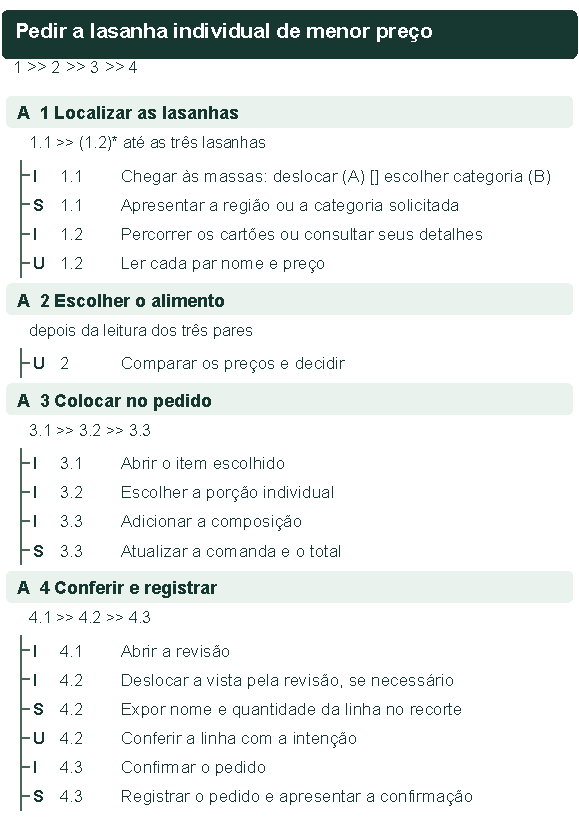
\includegraphics[width=\columnwidth]{../design/figures/CTT-C1.pdf}
\par\smallskip\noindent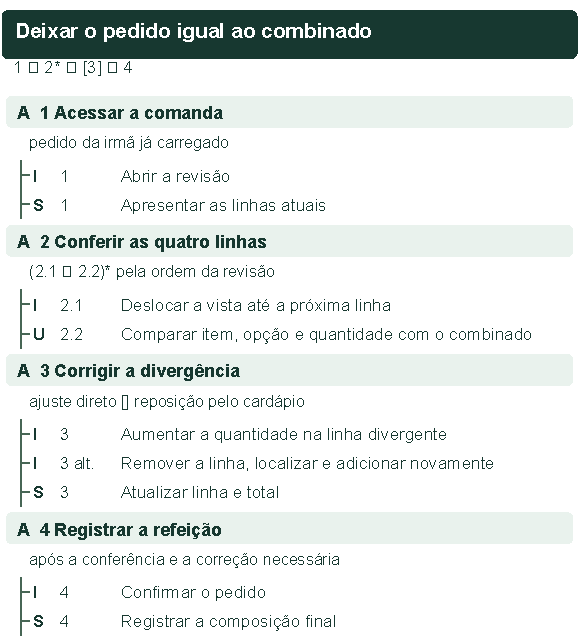
\includegraphics[width=\columnwidth]{../design/figures/CTT-C2.pdf}
\par\smallskip\noindent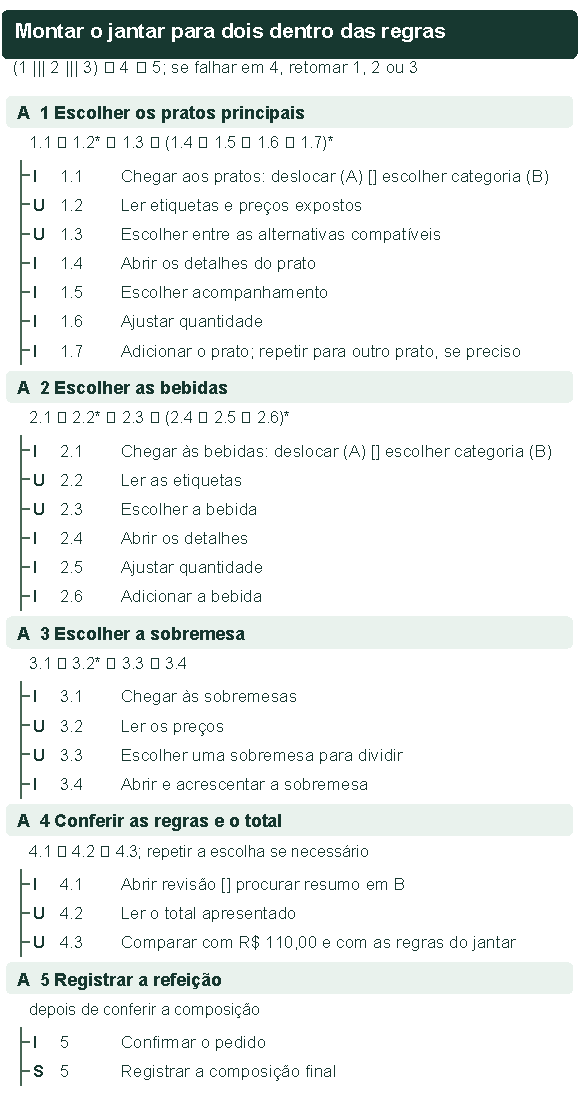
\includegraphics[width=\columnwidth]{../design/figures/CTT-V1.pdf}
\par\smallskip\noindent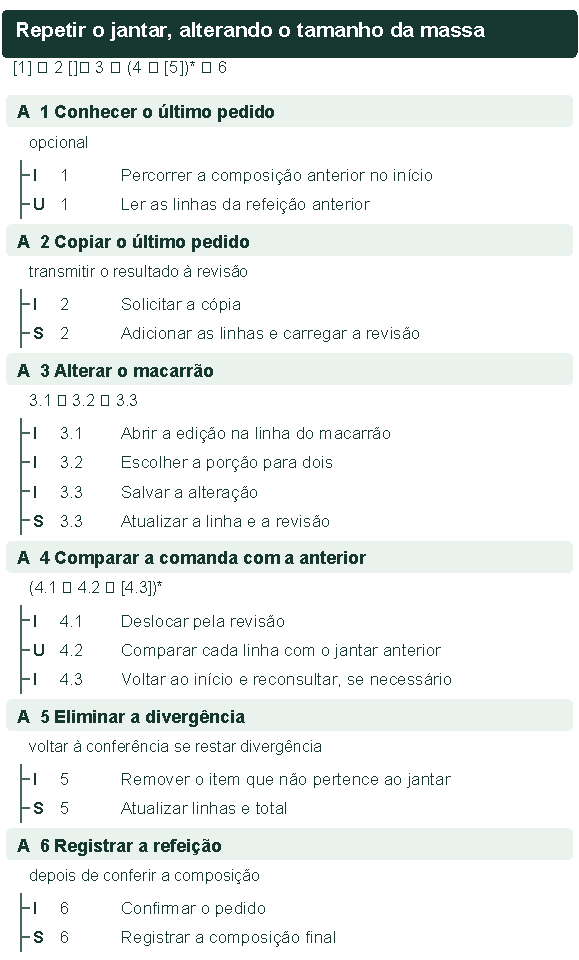
\includegraphics[width=\columnwidth]{../design/figures/CTT-V2.pdf}

\Etitle{Modelos GOMS e KLM}
\textit{CMN-GOMS de C1.} Objetivo: obter a lasanha individual de menor preço. Operadores observáveis: deslocar, abrir item, escolher porção, adicionar, abrir revisão, voltar e confirmar; comparar é operador interno. \emph{Método direto}: chegar às massas pela lista (A) ou pela categoria (B), ler três preços, abrir a escolhida, selecionar a porção individual, adicionar, rever e confirmar. \emph{Método por detalhes}: para cada preço ilegível, abrir o item, ler e voltar antes de decidir. \emph{Regra de seleção}: se o preço é legível junto do nome, usar o método direto; senão, o método por detalhes, que acrescenta uma abertura e um retorno por consulta. A escolha do método é observável e vira indicador: o registro conta as aberturas de S2 com retorno a S1 antes da primeira seleção de porção. No método direto há cinco toques em A ou seis em B, além dos deslocamentos determinados pela geometria. Em C2, alterar a unidade da linha exige menos operações que remover e recompor a linha; ambos são métodos admissíveis \cite[cap.~5, pp.~139--192]{card83}.
\par\textit{KLM na cena crítica.} Usa-se uma única tabela de tempos \cite[p.~399, Tabela~I]{card80}: apontar $P=1{,}10$~s, acionar $K=0{,}20$~s, preparar $M=1{,}35$~s. A aproximação de um toque por $PK$ é HO. O operador $M$ entra antes de cada escolha independente e nunca entre apontar e acionar o mesmo alvo, com o mesmo critério nas duas alternativas. Premissas: alvos localizados, sem deslocamento, resposta sem espera e especialista sem erro \cite[pp.~448--456]{preece}. Para consultar a composição durante a escolha e retomar a seleção, A exige abrir a revisão e voltar: $MPK\,MPK=5{,}30$~s. Em B, com o resumo na vista, a consulta não exige acionamento: $0$~s de operadores. A duração da leitura, presente nas duas alternativas, não é modelada; se o resumo sair da vista, a estimativa de B perde sua premissa. Na correção integral de C2 restam três escolhas nas duas versões: $3(MPK)=7{,}95$~s. O GOMS descreve o especialista sem erros: serve para comparar alternativas, definir o método de referência $N_{\rm ref}(z)$ que é denominador de $R_A$, detectar métodos inconsistentes e redigir a ajuda procedimental. Não é modelo da persona, e usar esses tempos como duração de uma pessoa novata com baixa visão seria HO sem sustentação. HTA, CTT e GOMS ficam com o analista; nenhum deles é entregue ao agente.


\Etitle{Diagrama MoLIC}
As cenas delimitam assuntos, P identifica processos e as guardas limitam atos de fala. O subdiálogo S5 preserva a cena de origem; ajustar a vista conserva o assunto corrente; a desistência encerra a sessão.
\par\smallskip\noindent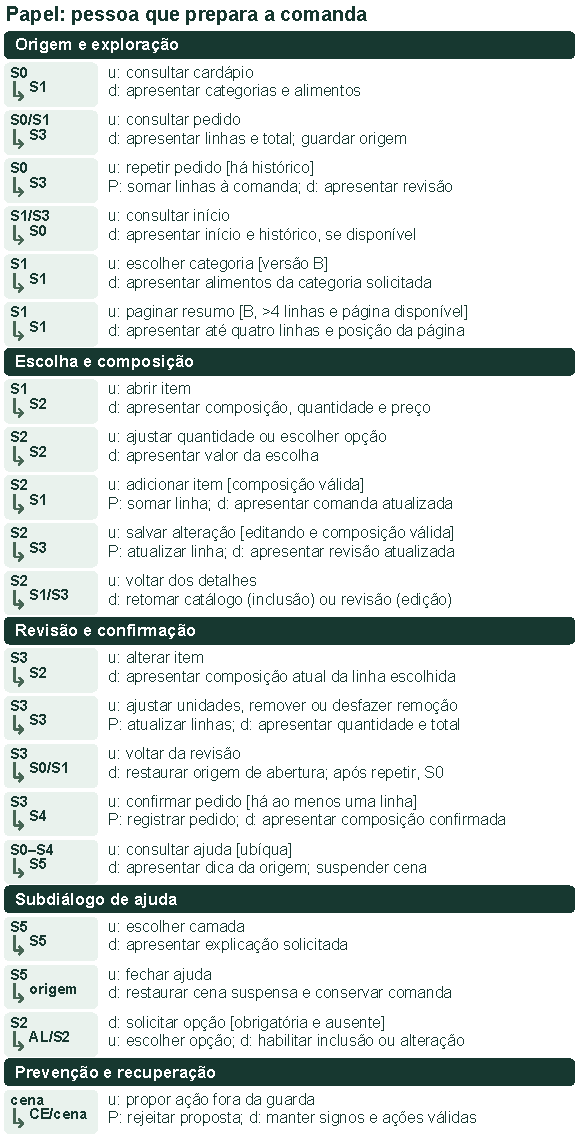
\includegraphics[width=\columnwidth]{../design/figures/MoLIC.pdf}
\par\smallskip
A MoLIC representa o único papel de usuário, quem faz o pedido \cite{molic}. As falas u: de uma cena são as ações disponíveis ao executor naquele estado; a fala d: seguinte é o conteúdo da próxima observação. A conclusão (d: OK) é condição de estado avaliada pelo verificador externo, nunca pela declaração do agente. Como a MoLIC não é modelo formal processável, o executor processa o statechart da Fig.~\ref{fig:estados}, no qual a ajuda é um subdiálogo que devolve a pessoa à cena de origem. A Tabela~\ref{tab:molic} dá as três leituras de cada elemento.
\begin{figure}[ht]
\centering
\setlength{\unitlength}{1pt}
\begin{picture}(238,112)
\put(0,87){\framebox(50,18){S0 · Início}}
\put(94,87){\framebox(58,18){S1 · Cardápio}}
\put(188,87){\framebox(48,18){S2 · Item}}
\put(50,98){\vector(1,0){44}}\put(59,101){\scriptsize abrir}
\put(94,91){\vector(-1,0){44}}\put(57,80){\scriptsize início}
\put(152,98){\vector(1,0){36}}\put(154,101){\scriptsize escolher}
\put(188,91){\vector(-1,0){36}}\put(157,80){\scriptsize incluir}
\put(94,40){\framebox(58,18){S3 · Revisão}}
\put(188,40){\framebox(48,18){S4 · Fim}}
\put(123,87){\vector(0,-1){29}}\put(127,69){\scriptsize rever}
\put(113,58){\vector(0,1){29}}\put(64,68){\scriptsize continuar}
\put(152,48){\vector(1,0){36}}\put(151,53){\scriptsize confirmar}
\put(212,87){\line(0,-1){24}}\put(212,63){\line(-1,0){73}}\put(139,63){\vector(0,-1){5}}\put(172,66){\scriptsize salvar}
\put(25,87){\line(0,-1){39}}\put(25,48){\vector(1,0){69}}\put(30,51){\scriptsize repetir ou rever}
\put(0,4){\framebox(101,18){Origem · S0 a S4}}
\put(158,4){\framebox(78,18){S5 · Ajuda}}
\put(101,17){\vector(1,0){57}}\put(110,21){\scriptsize consultar}
\put(158,9){\vector(-1,0){57}}\put(116,0){\scriptsize fechar}
\end{picture}
\caption{Transições principais da implementação. Editar uma linha em S3 reabre S2. Voltar preserva a origem da revisão ou da edição. Confirmar exige comanda não vazia. Uma fala inválida mantém a cena; o suporte restaura a origem.}
\label{fig:estados}
\end{figure}

\begin{table*}[!t]
\caption{Leituras de cada elemento da MoLIC}
\label{tab:molic}
\centering\scriptsize\setlength{\tabcolsep}{3pt}\renewcommand{\arraystretch}{1.1}
\begin{tabularx}{\textwidth}{@{}>{\raggedright\arraybackslash}p{.11\textwidth}>{\raggedright\arraybackslash}X>{\raggedright\arraybackslash}X>{\raggedright\arraybackslash}p{.25\textwidth}@{}}
\hline \textbf{Elemento MoLIC} & \textbf{Leitura da persona} & \textbf{Leitura do agente (observação ou ação)} & \textbf{Evento registrado}\\ \hline
Cena & Reconhece o assunto (início, cardápio, item, revisão, fim, ajuda) pelos signos da tela. & Observação: título e signos da cena que cruzam o recorte. & \UXev{tela_alterada} com cena anterior e nova\\
Fala u: & Solicita uma operação, como abrir um item, alterar a quantidade ou confirmar. & Ação: um gesto permitido sobre um alvo exposto, escolhido entre as alternativas do estado. & \UXev{acao_proposta}, \UXev{acao_executada}; proposta inválida: \UXev{acao_rejeitada}\\
Fala d: & Vê a resposta do preposto, como a nova quantidade da linha e o novo total. & Observação seguinte: o fragmento exposto da resposta. & \UXev{elemento_visto} e o evento de mutação correspondente\\
Processo do sistema & Percebe o efeito: comanda copiada, recalculada ou registrada. & Observação do efeito expresso; o estado integral fica com o verificador. & \UXev{item_adicionado}, \UXev{item_alterado}, \UXev{item_removido}, \UXev{pedido_confirmado}\\
Fala de recuperação & Volta aos detalhes, recompõe a linha, remove ou desfaz a remoção. & As mesmas ações de recuperação, quando expostas. & \UXev{item_alterado}, \UXev{item_removido}, \UXev{item_adicionado}\\
Acesso ubíquo à ajuda & Abre a ajuda em qualquer cena, escolhe a camada e fecha para voltar à origem. & Ação de protocolo sempre disponível; o conteúdo só chega após a abertura. & \UXev{ajuda_aberta} e \UXev{ajuda_fechada} com camada, tópico, origem e retorno\\ \hline
\end{tabularx}
\end{table*}



\Etitle{Matriz de prevenção e recuperação de erros (PP, PA, AL, RA, CE)}
PP antecipa um problema pela expressão, PA restringe uma operação, AL alerta, RA permite corrigir e CE captura uma tentativa inválida. As operações seguem a numeração da HTA \cite[pp.~5, 8--9]{hts}. Toda PP tem RA equivalente e a única PA, sobre a inclusão sem opção, vem com PP (Tabela~\ref{tab:rupturas}). Com PA o erro deixa de ocorrer; com PP e RA ele ocorre e é registrado, mesmo quando recuperado. As taxas exigem guardas e denominadores equivalentes no comparador humano. Alertas sobre uma divergência específica entregariam o critério da tarefa; a interface informa apenas valores e operações.
\begin{table*}[!t]
\caption{Matriz de prevenção e recuperação de rupturas por operação da HTA}
\label{tab:rupturas}
\centering\scriptsize\setlength{\tabcolsep}{3pt}\renewcommand{\arraystretch}{1.1}
\begin{tabularx}{\textwidth}{@{}>{\raggedright\arraybackslash}p{.15\textwidth}>{\raggedright\arraybackslash}p{.12\textwidth}>{\raggedright\arraybackslash}p{.11\textwidth}>{\raggedright\arraybackslash}X>{\raggedright\arraybackslash}p{.17\textwidth}>{\raggedright\arraybackslash}p{.1\textwidth}@{}}
\hline \textbf{Operação da HTA} & \textbf{Erro previsto} & \textbf{Mecanismo} & \textbf{Signo} & \textbf{Evento} & \textbf{Métrica}\\ \hline
C1\,1; C2\,2.1; V1\,1--3; V2\,4.1 & deslize ou omissão de item & PP + RA & nome e preço agrupados (PP); reconsultar ou voltar (RA) & \UXev{vista_deslocada}, \UXev{elemento_visto}, \UXev{deslize_injetado} & $D$, $O$, $Re_{E4}$, $A$\\
C1\,2--3.1; V1\,1--3; V2\,3.1 e 5 & seleção ou associação errada & PP + RA & nome junto do preço, etiquetas e controles (PP); rever, remover ou recompor (RA) & \UXev{item_adicionado}, \UXev{item_alterado}, \UXev{item_removido} & $Re_{E1}$, $Re_{E2}$, $V$\\
C1\,3.2--3.3; C2\,3; V1\,1.5--1.7 e 2.5--2.6; V2\,3.2--3.3 & opção ausente ou quantidade errada & PP + PA + RA & opção exigida e número expostos (PP); inclusão bloqueada sem opção (PA); escolher e editar (RA) & \UXev{opcao_selecionada}, \UXev{item_alterado} & $Re_{E3}$\\
C1\,4; C2\,2.2--4; V2\,4--6 & divergência confirmada & PP + RA & linhas e total antecipam a consequência (PP); alterar quantidade, reconsultar ou remover (RA) & \UXev{elemento_visto}, \UXev{pedido_confirmado} & $Re_{E5}$, $O$\\
V1\,4--5 & regra ou orçamento violado & PP + RA & etiquetas e total (PP); substituir antes de confirmar (RA) & \UXev{pedido_confirmado} & $Re_{E6}$\\
Todas & fala fora do conjunto permitido & CE + AL & a guarda captura a proposta (CE); o aviso de opção necessária alerta (AL) & \UXev{acao_rejeitada}, \UXev{elemento_visto} & rejeições, fora de $A$\\ \hline
\end{tabularx}
\end{table*}



\Etitle{Identificação de rupturas comunicativas (MAC)}
Seis etiquetas do MAC \cite{mac} são definidas como padrões de eventos (Tabela~\ref{tab:mac}). Cada definição é HO: o padrão no registro do agente não equivale à experiência de ruptura de uma pessoa. Duas assinaturas podem coincidir, e a mesma definição será aplicada aos dados humanos quando houver registros compatíveis.
\begin{table}[!t]
\caption{Etiquetas MAC operacionalizadas como padrões de eventos (HO)}
\label{tab:mac}
\centering\scriptsize\setlength{\tabcolsep}{3pt}\renewcommand{\arraystretch}{1.1}
\begin{tabularx}{\columnwidth}{@{}>{\raggedright\arraybackslash}p{.27\columnwidth}>{\raggedright\arraybackslash}X@{}}
\hline \textbf{Etiqueta} & \textbf{Padrão no registro}\\ \hline
\emph{Socorro!} & \UXev{ajuda_aberta}, por ação da pessoa ou do acionador M7.\\
\emph{O que é isso?} & \UXev{ajuda_aberta} na primeira camada (dica local) para um tópico.\\
\emph{Desisto} & \UXev{desistencia} por ação explícita.\\
\emph{Pra mim está bom} & \UXev{pedido_confirmado} seguido de resultado de fracasso no verificador.\\
\emph{Epa!} & \UXev{deslize_injetado} seguido, em até duas ações executadas, de retorno ou correção aplicável.\\
\emph{Cadê?} & $n=5$ ações executadas seguidas sem novo signo, nova cena ou mutação do pedido; uma ocorrência por sequência.\\ \hline
\end{tabularx}
\end{table}



\Etitle{Mecanismos de ajuda}
A ajuda é a metacomunicação explícita do designer e também variável de protocolo. Seu conteúdo procede dos conceitos, das tarefas e da conversa \cite[pp.~39--55]{silveira} (Tabela~\ref{tab:duvidas}). S5 é contextual, em três camadas e sob demanda: \emph{dica local}, \emph{sobre esta tela} e \emph{guia de uso}. O acesso fica no botão Ajuda de cada cena e no atalho F1; a pessoa escolhe a camada e fecha para voltar à origem.
\begin{table*}[!t]
\caption{Conteúdo da ajuda a partir dos tipos de dúvida}
\label{tab:duvidas}
\centering\scriptsize\setlength{\tabcolsep}{3pt}\renewcommand{\arraystretch}{1.1}
\begin{tabularx}{\textwidth}{@{}>{\raggedright\arraybackslash}p{.11\textwidth}>{\raggedright\arraybackslash}p{.2\textwidth}>{\raggedright\arraybackslash}p{.15\textwidth}>{\raggedright\arraybackslash}X@{}}
\hline \textbf{Dúvida} & \textbf{Pergunta} & \textbf{Modelo de origem} & \textbf{Conteúdo}\\ \hline
Informativa & O que o restaurante oferece? & domínio, S1 & Cada item tem nome, descrição e preço.\\
Descritiva & O que é tamanho? & signos, S2 & Tamanho é a porção da massa, distinto da quantidade.\\
Procedimental & Como editar uma linha? & GOMS, S2/S3 & Alterar a linha, escolher a opção e salvar.\\
De escolha & Alterar ou remover? & MoLIC, S3 & Alterar edita as opções; remover retira a linha.\\
Sugestiva & O que conferir? & cenário, S3 & Conferir nomes, opções e quantidades.\\
Investigativa & Onde vejo o efeito? & processo, S3 & A quantidade e o total expressam a mudança.\\
Interpretativa & O que é SA? & domínio, S1 & Sem açúcar ou sem açúcar adicionado.\\
Navegacional & Onde rever o pedido? & MoLIC, S1 & A revisão reúne as linhas em andamento.\\
Histórica & O que foi repetido? & comanda, S0 & Reconsultar a composição anterior e conferir a cópia.\\
De motivação & Por que confirmar? & metamensagem, S4 & Confirmar registra e encerra o pedido.\\ \hline
\end{tabularx}
\end{table*}
\par\textit{Requisitos de Dix} \cite[pp.~397--399]{dix}. Disponibilidade: acesso em todas as cenas da interação. Precisão e completude: cada tópico descreve operações existentes e as camadas cobrem as dez dúvidas. Consistência: títulos e orientações usam o vocabulário das ações. Robustez: ler não altera o pedido e fechar retorna à origem. Flexibilidade: a pessoa escolhe a profundidade. Discrição: o conteúdo só aparece após a abertura.
\par\textit{Registro e uso de suporte.} Cada acesso gera \UXev{ajuda_aberta} com camada, tópico, cena de origem e origem da solicitação; fechar gera \UXev{ajuda_fechada} com o retorno. Para cada camada, $U$ conta acessos por execução e a fração das execuções elegíveis com acesso (denominador: execuções iniciadas sem falha técnica). A posição do primeiro acesso é o índice da ação dividido pelo número de ações executadas.
\par\textit{Igualdade e congelamento.} Uma única fonte textual atende a interface humana e a projeção do agente, que só recebe o conteúdo depois da abertura. A ajuda não é adaptativa. Na calibração (C1/C2) é permitido inspecionar entradas e saídas e comparar o acionador M7 ligado e desligado; na validação (V1/V2) conteúdo, camadas e parâmetros ficam congelados. A interface não tem agente de ajuda: M7 pertence ao controlador que representa a persona, do outro lado da interface, e sua solicitação é registrada com origem \texttt{acionador}.

\par\smallskip\noindent\textit{Texto das três camadas, por cena.}
\par\smallskip\noindent\textbf{S0}
\par\noindent\emph{Dica local.} Consulte o cardápio para começar. Se houver um último pedido, você pode consultá-lo aqui.
\par\noindent\emph{Sobre esta tela.} O último pedido mostra a composição registrada anteriormente. Repetir pedido acrescenta esses itens ao pedido em andamento. Confira também os itens que já estavam nele.
\par\noindent\emph{Guia de uso.} Para começar de novo pelo cardápio, escolha Ver cardápio. Para usar uma composição anterior, escolha Repetir pedido, se disponível. Na revisão, confira as opções e as quantidades. O pedido é registrado quando você o confirma.
\par\smallskip\noindent\textbf{S1}
\par\noindent\emph{Dica local.} Cada item tem nome, descrição e preço. Consulte o item para conhecer as opções disponíveis.
\par\noindent\emph{Sobre esta tela.} Na lista contínua, os itens aparecem por categoria. Na versão com categorias, escolha o nome da categoria para ver seus itens. Ver pedido abre a revisão. O resumo no rodapé, quando presente, acompanha o pedido em andamento.
\par\noindent\emph{Guia de uso.} As etiquetas pertencem ao item junto do qual aparecem. (V) significa vegetariano, (SL) significa sem lactose e (SA) significa sem açúcar ou sem açúcar adicionado. Consulte os detalhes, escolha as opções desejadas e acrescente o item. Você pode rever o pedido antes de confirmar.
\par\smallskip\noindent\textbf{S2}
\par\noindent\emph{Dica local.} Confira o nome e o preço do item. Quando houver uma opção obrigatória, escolha-a antes de acrescentar ou salvar.
\par\noindent\emph{Sobre esta tela.} O acompanhamento compõe o prato principal. O tamanho define a porção de massa. A quantidade indica quantas unidades da combinação serão pedidas. Aumente ou diminua a quantidade pelos controles junto ao número.
\par\noindent\emph{Guia de uso.} Ao incluir um item, escolha a opção, ajuste a quantidade e use Adicionar. Ao modificar uma linha existente, use Salvar alteração. Para sair dos detalhes antes de aplicar a escolha, use Voltar.
\par\smallskip\noindent\textbf{S3}
\par\noindent\emph{Dica local.} Confira cada linha, suas opções e quantidades. O total reúne todas as linhas do pedido.
\par\noindent\emph{Sobre esta tela.} Use os controles junto à quantidade para ajustá-la. Alterar permite rever as opções da linha. Remover retira a linha do pedido. Confira o nome junto dos controles antes de fazer uma alteração.
\par\noindent\emph{Guia de uso.} Percorra o pedido e confira as linhas com o que deseja receber. Para recuperar uma linha, use Desfazer remoção enquanto essa opção estiver disponível. Você também pode voltar ao cardápio e acrescentar o item novamente. Ao terminar a conferência, use Confirmar pedido.
\par\smallskip\noindent\textbf{S4}
\par\noindent\emph{Dica local.} A confirmação indica que o pedido foi registrado.
\par\noindent\emph{Sobre esta tela.} O registro conclui a composição do pedido neste restaurante fictício. A confirmação informa que a operação terminou.
\par\noindent\emph{Guia de uso.} Consulte a mensagem de confirmação para reconhecer o fim do pedido. Esta demonstração não processa pagamentos nem envia pedidos a restaurantes.

